
%(BEGIN_QUESTION)
% Copyright 2010, Tony R. Kuphaldt, released under the Creative Commons Attribution License (v 1.0)
% This means you may do almost anything with this work of mine, so long as you give me proper credit

A {\it Pirani gauge} is a special pressure instrument designed to measure very low pressures (i.e. hard vacuums).  It uses two electrically heated filaments, one of which is dealed in a vacuum ``reference'' chamber, while the other is exposed to the process gas pressure under test.  Gas molecules contacting the measurement filament causes it to cool and decrease resistance:

$$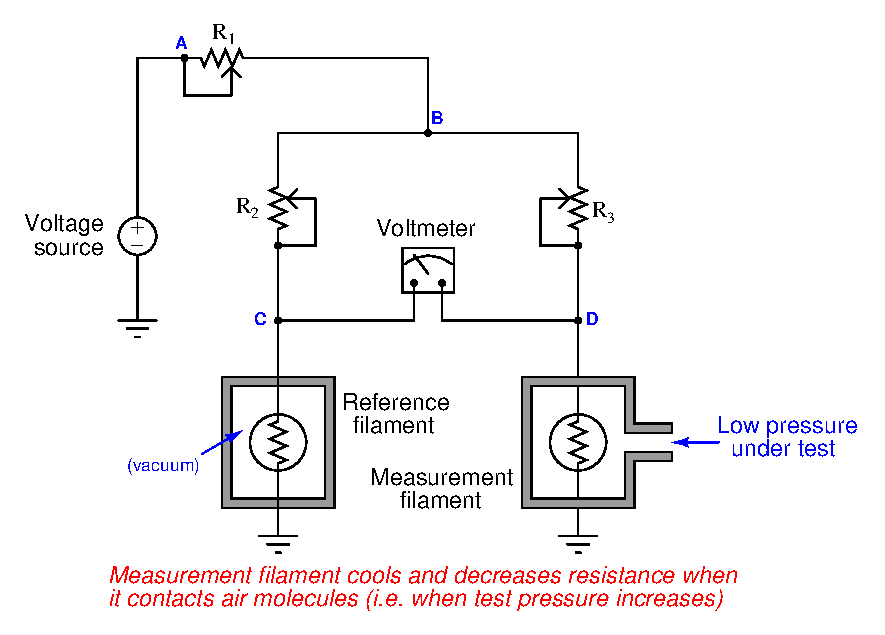
\includegraphics[width=15.5cm]{i00300x01.eps}$$

This Pirani gauge, however, has a problem.  It registers a high pressure all the time, regardless of the strength of the vacuum connected to the measurement cell.  A digital multimeter connected between test points {\bf D} and ground registers 0 volts.

Identify the likelihood of each specified fault for this circuit.  Consider each fault one at a time (i.e. no coincidental faults), determining whether or not each fault could independently account for {\it all} measurements and symptoms in this circuit.

% No blank lines allowed between lines of an \halign structure!
% I use comments (%) instead, so that TeX doesn't choke.

$$\vbox{\offinterlineskip
\halign{\strut
\vrule \quad\hfil # \ \hfil & 
\vrule \quad\hfil # \ \hfil & 
\vrule \quad\hfil # \ \hfil \vrule \cr
\noalign{\hrule}
%
% First row
{\bf Fault} & {\bf Possible} & {\bf Impossible} \cr
%
\noalign{\hrule}
%
% Another row
$R_1$ failed open &  &  \cr
%
\noalign{\hrule}
%
% Another row
$R_1$ failed shorted &  &  \cr
%
\noalign{\hrule}
%
% Another row
$R_2$ failed open &  &  \cr
%
\noalign{\hrule}
%
% Another row
$R_2$ failed shorted &  &  \cr
%
\noalign{\hrule}
%
% Another row
$R_3$ failed open &  &  \cr
%
\noalign{\hrule}
%
% Another row
$R_3$ failed shorted &  &  \cr
%
\noalign{\hrule}
%
% Another row
Reference filament burned out &  &  \cr
%
\noalign{\hrule}
%
% Another row
Measurement filament burned out &  &  \cr
%
\noalign{\hrule}
} % End of \halign 
}$$ % End of \vbox


\underbar{file i00300}
%(END_QUESTION)





%(BEGIN_ANSWER)

% No blank lines allowed between lines of an \halign structure!
% I use comments (%) instead, so that TeX doesn't choke.

$$\vbox{\offinterlineskip
\halign{\strut
\vrule \quad\hfil # \ \hfil & 
\vrule \quad\hfil # \ \hfil & 
\vrule \quad\hfil # \ \hfil \vrule \cr
\noalign{\hrule}
%
% First row
{\bf Fault} & {\bf Possible} & {\bf Impossible} \cr
%
\noalign{\hrule}
%
% Another row
$R_1$ failed open &  & $\surd$ \cr
%
\noalign{\hrule}
%
% Another row
$R_1$ failed shorted &  & $\surd$ \cr
%
\noalign{\hrule}
%
% Another row
$R_2$ failed open &  & $\surd$ \cr
%
\noalign{\hrule}
%
% Another row
$R_2$ failed shorted &  & $\surd$ \cr
%
\noalign{\hrule}
%
% Another row
$R_3$ failed open & $\surd$ &  \cr
%
\noalign{\hrule}
%
% Another row
$R_3$ failed shorted &  & $\surd$ \cr
%
\noalign{\hrule}
%
% Another row
Reference filament burned out &  & $\surd$ \cr
%
\noalign{\hrule}
%
% Another row
Measurement filament burned out &  & $\surd$ \cr
%
\noalign{\hrule}
} % End of \halign 
}$$ % End of \vbox


%(END_ANSWER)





%(BEGIN_NOTES)


\filbreak \vskip 20pt \vbox{\hrule \hbox{\strut \vrule{} {\bf Virtual Troubleshooting} \vrule} \hrule}

\noindent
{\bf Predicting the effect of a given fault:} present each of the following faults to the students, one at a time, having them comment on all the effects each fault would produce.

\begin{itemize}
\item{} R1 fails open
\item{} R1 fails shorted
\item{} R2 fails open
\item{} R2 fails shorted
\item{} R3 fails open
\item{} R3 fails shorted
\item{} Reference filament fails open
\item{} Reference filament fails shorted
\item{} Measurement filament fails open
\item{} Measurement filament fails shorted
\end{itemize}


\vskip 10pt


\noindent
{\bf Identifying possible/impossible faults:} present symptoms to the students and then have them determine whether or not a series of suggested faults could account for all the symptoms, explaining {\it why} or {\it why not} for each proposed fault:

\begin{itemize}
\item{} Symptom: {\it }
\item{}  -- {\bf Yes/No}
\item{}  -- {\bf Yes/No}
\item{}  -- {\bf Yes/No}
\end{itemize}


\vskip 10pt


\noindent
{\bf Determining the utility of given diagnostic tests:} present symptoms to the students and then propose the following diagnostic tests one by one.  Students rate the value of each test, determining whether or not it would give useful information (i.e. tell us something we don't already know).  Students determine what different results for each test would indicate about the fault, if anything:

\begin{itemize}
\item{} Symptom: {\it }
\item{}  -- {\bf Yes/No}
\item{}  -- {\bf Yes/No}
\end{itemize}


\vskip 10pt


\noindent
{\bf Diagnosing a fault based on given symptoms:} imagine the reference filamant fails open in this system (don't reveal the fault to students!).  Present the operator's observation(s) to the students, have them consider possible faults and diagnostic strategies, and then tell them the results of tests they propose based on the following symptoms, until they have properly identified the nature and location of the fault:

\begin{itemize}
\item{} Operator observation: {\it gauge registers a high pressure all the time}
\item{} $V_A$ normal
\item{} $V_B$ slightly greater than normal
\item{} $V_C$ much greater than normal
\item{} $V_D$ slightly greater than normal
\end{itemize}

%INDEX% Measurement, pressure: Pirani gauge
%INDEX% Troubleshooting review: electric circuits

%(END_NOTES)


